\subsection{Smallest measurable translational force}
\label{sec:Smallestmeasurable}

The smallest measurable translational force can be obtained with geometry. The pendulum forms a right triangle where the vertical line is the pole itself \textit{"L"}, the horizontal is the ruler \textit{"x"} and the hypotenuse is the pendulum's string as depicted on figure \ref{fig:triangleDiagram}. Both of these measurements have a $1mm$ precision, yielding a L=1m and z=1mm triangle. Then, the smallest deflection angle capable of measurement is given by $\alpha=\tan(z/L) \sim z/L$ for small angle which is about of a $10^{-3}$ rad ($\sim$ 0.057 deg). 
\begin{wrapfigure}{r}{0.35\textwidth}
	%\vspace{-30pt}
	\centering
	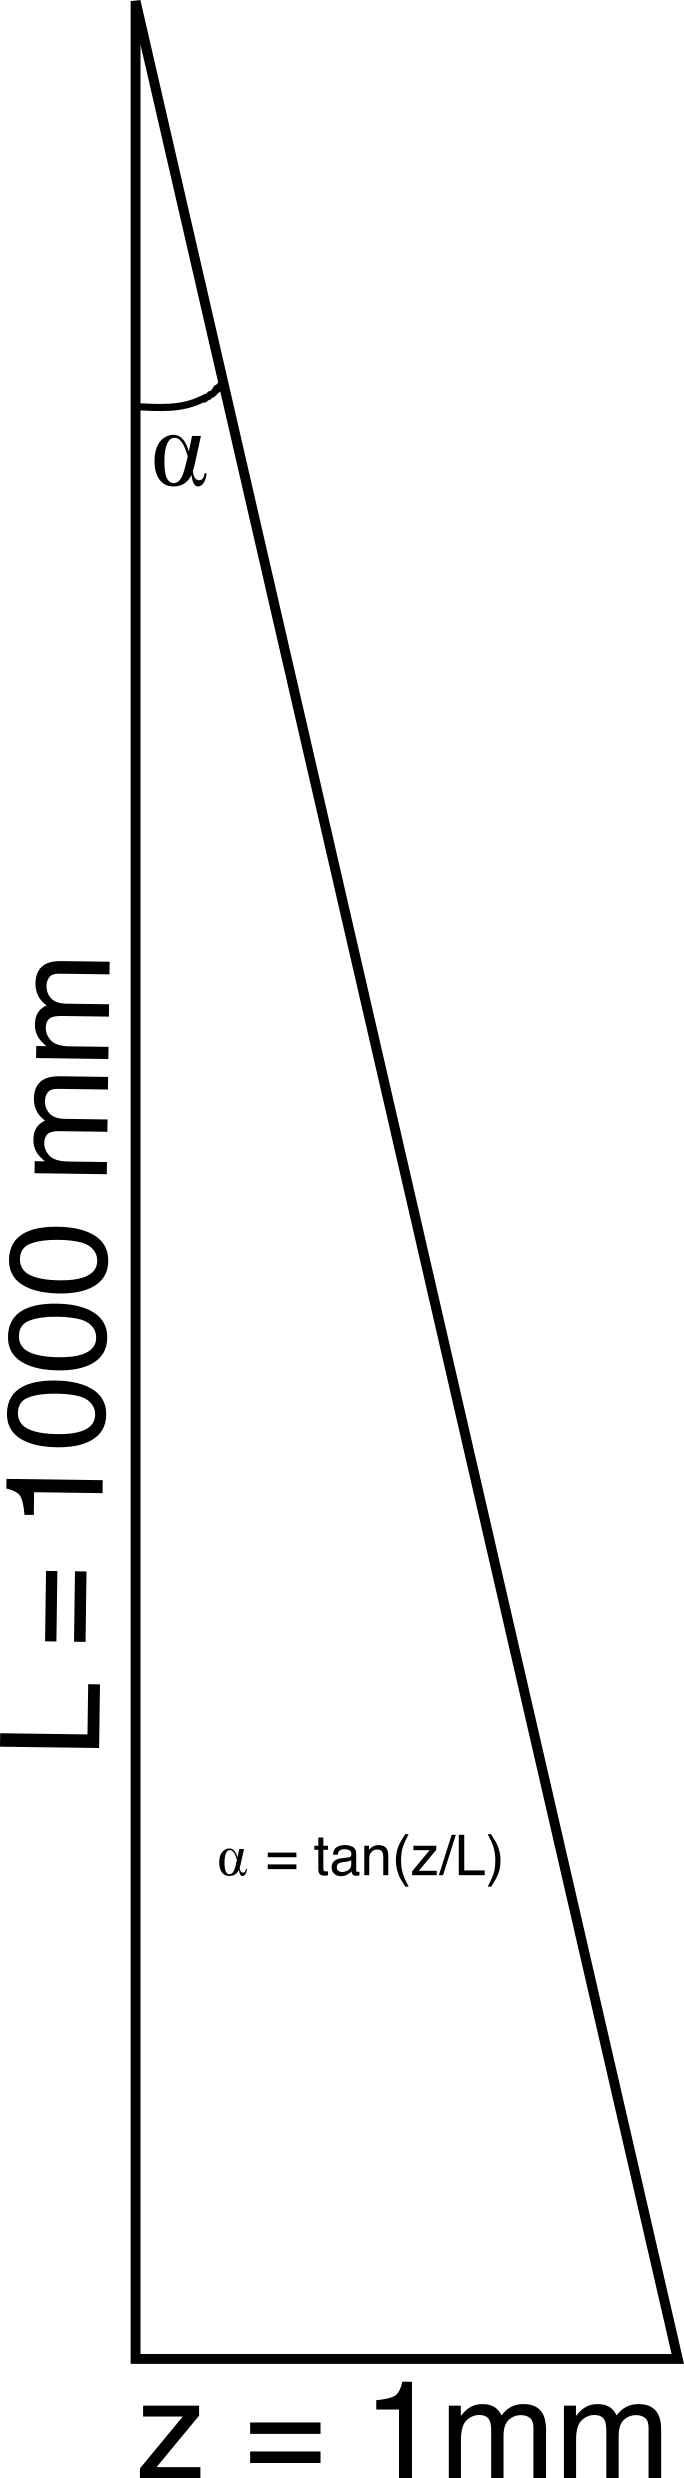
\includegraphics[width=0.15\textwidth]{Assets/leastmeasure.png}
	\caption{Right-angled triangle formed by the pendulum geometry at equilibrium.}
	\label{fig:triangleDiagram}
	%\vspace{10pt}
\end{wrapfigure}

Since the angular deflection corresponds to the ratio of magnetic to gravitational forces (see eq. \ref{eq:deflectionAngle}) the smallest measurable magnetic force is 

\begin{equation}
	\label{eq:minForce}
	F_{m,min} = \tan(\alpha_{min})= mg (\frac{z}{L}).
\end{equation}

For a 1g test mass\footnote{Sample calculations can be found on appendix \ref{app:smallestForce}}, this corresponds to a detection threshold of $F_{m,min} \sim 10^{-6}N$ ($1\mu N$). Thus, the apparatus can resolve magnetic force as small as one-thousandth of the object’s weight. This resolution defines the lower limit of measurable magnetic susceptibility using the pendulum method. For nonmagnetic or weakly paramagnetic materials, such sensitivity ensures that even subtle translational forces can be quantified, making the setup suitable for assessing device safety under MRI static field gradients.